\usepackage[utf8]{inputenc}
\usepackage[T1]{fontenc}
\usepackage{lmodern}

% shift material to outer margin for physical copies
\newif\ifpaper
%\papertrue
\paperfalse

\ifpaper
  \newcommand{\horizontalOffset}{0.365in} %
  \newcommand{\horizontalOffsetInPts}{26pt} % = inches * 72.27
  \usepackage[margin=1.5in,inner=1.8in,outer=1.2in]{geometry} %
\else
  \newcommand{\horizontalOffset}{0in} %
  \newcommand{\horizontalOffsetInPts}{0pt} % = inches * 72.27
  \usepackage[margin=1.5in]{geometry} %
\fi

\usepackage{tocloft}     % to typeset ToC 
\usepackage[hyphens]{url}% to typeset URLs, URIs, and DOIs; allow breaking at hyphens
\usepackage{listings}    % to create code listings
\usepackage{graphicx}    % to include graphics
\usepackage{svg}         % to include svg images
\usepackage{tikz}        % to include .tex graphics
\usepackage{eso-pic}     % to include .pdf as bg image
\usepackage{caption}     % to jump to start of Figures etc., on clicking a reference to them, rather than to their caption
%\usepackage[table]{xcolor} % to add colour to tables
\usepackage{tabto}           % to add tabs 
\usepackage{amsthm, amssymb} % to include definition environment
\usepackage[most]{tcolorbox}  % to create definition boxes
%\usepackage{lstlinebgrd} % to add highlighting to listings
\usepackage{chapterbib}   % to have a bibliography per chapter
\usepackage{etoolbox} % to format block quotes
\usepackage{setspace} % to format line spacing
\usepackage[unicode=true]{hyperref} % to typeset hrefs
\usepackage{bookmark} % to be able to exclude a Chapter from a Part (e.g., Conclusion)
\usepackage[font=small]{caption}  % to have small font captions
\usepackage[strict]{changepage} % to check odd/even pages
\usepackage{enumitem}  % to enumerate using alphabet
\usepackage{rotating}  % to rotate figures
\usepackage{booktabs}  % to thicken table lines
\usepackage{longtable} % to allow tables spanning multiple pages
\usepackage{multirow}  % to use multirow cells
%\usepackage{easyReview} % to add review comments
\usepackage{pdfpages}  % to include pdfs
\usepackage{appendix}  % to have appendices per chapter
\usepackage{chngcntr}  % to have appendices per chapter
\usepackage{etoolbox}  % to have appendices per chapter
\usepackage{ragged2e}  % to include RaggedRight command
\def\UrlFont{\rmfamily}

\setcounter{tocdepth}{0}

% avoid all hyphenation
%\tolerance=1
%\emergencystretch=\maxdimen
%\hyphenpenalty=10000
%\hbadness=10000

% lower hyphenation to acceptable levels
\pretolerance=5000
\tolerance=9000
\emergencystretch=0pt
\righthyphenmin=4
\lefthyphenmin=4

%  handle spacing between sentences in the same way as spacing between words in the middle of a sentence
\frenchspacing 

% avoid spacing between paragraphs just to fill out a page
\raggedbottom

% ensuring spacing of block quotes
\AtBeginEnvironment{quote}{\par\singlespacing\small}

% border/line color of tables
\arrayrulecolor{lightgray}

% define custom colours
\definecolor{evokeblue}{RGB}{26, 167, 224}
\definecolor{evokelightblue}{RGB}{112, 193, 224}

% define \convertto command, converting a length from one unit of measure to another, see http://groups.google.com/group/comp.text.tex/msg/7e812e5d6e67fcc5
%\def\convertto#1#2{\strip@pt\dimexpr #2*65536/\number\dimexpr 1#1}

% define \hr command
%\newcommand\hr{\par\vspace{-.5\ht\strutbox}\noindent\hrulefill\par}

% define \lbl command
\newcommand{\lbl}[1]{\setlength{\fboxrule}{0em}\fcolorbox{gray!20}{gray!20}{#1}}

% define \BackgroundPicTitle command
\newcommand\BackgroundPicTitle{
    \put(0,0){
    \parbox[b][\paperheight]{\paperwidth}{%
    \vfill
    \centering
    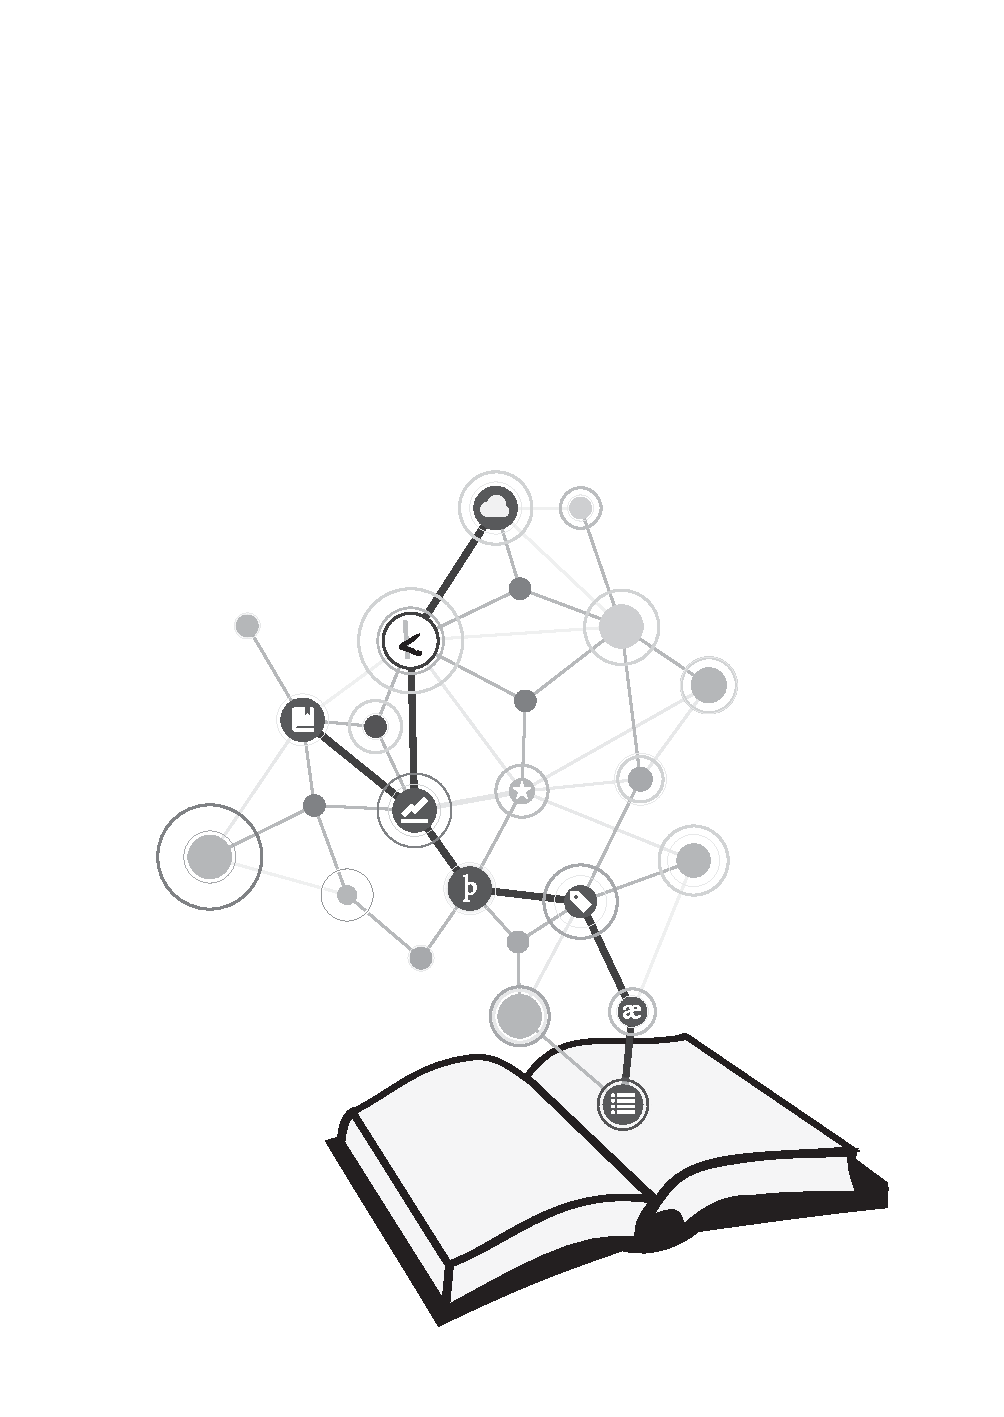
\includegraphics[width=\paperwidth,height=\paperheight]{apparatus/fig/coverimg-greyscale.pdf}
    \vfill
    }}}

% adjust layout of table of contents
\renewcommand{\cftpartfont}{\bfseries\color{evokeblue}}
\renewcommand{\cftpartpagefont}{\color{evokeblue}}
\renewcommand{\cftchapfont}{\normalfont}
\renewcommand{\cftchappagefont}{\normalfont}
\setlength{\cftbeforechapskip}{0.5em}
%\cftpagenumbersoff{part}
\cftsetrmarg{5em}


% set url colour
\hypersetup{
  colorlinks=true,
  linkcolor=black, 
  urlcolor=evokeblue
}

% set properties of lstlisting
\lstset{
	numberbychapter=false,
	frame = single,
	tabsize = 4,
	escapeinside = {(*@}{@*)},
	basicstyle=\normalsize\ttfamily,
	columns=fullflexible,
	aboveskip=15pt,
	belowskip=10pt,
	extendedchars=true,
    texcl=true,
    literate=
  {á}{{\'a}}1 {é}{{\'e}}1 {í}{{\'i}}1 {ó}{{\'o}}1 {ú}{{\'u}}1
  {Á}{{\'A}}1 {É}{{\'E}}1 {Í}{{\'I}}1 {Ó}{{\'O}}1 {Ú}{{\'U}}1
  {à}{{\`a}}1 {è}{{\`e}}1 {ì}{{\`i}}1 {ò}{{\`o}}1 {ù}{{\`u}}1
  {À}{{\`A}}1 {È}{{\'E}}1 {Ì}{{\`I}}1 {Ò}{{\`O}}1 {Ù}{{\`U}}1
  {ä}{{\"a}}1 {ë}{{\"e}}1 {ï}{{\"i}}1 {ö}{{\"o}}1 {ü}{{\"u}}1
  {Ä}{{\"A}}1 {Ë}{{\"E}}1 {Ï}{{\"I}}1 {Ö}{{\"O}}1 {Ü}{{\"U}}1
  {â}{{\^a}}1 {ê}{{\^e}}1 {î}{{\^i}}1 {ô}{{\^o}}1 {û}{{\^u}}1
  {Â}{{\^A}}1 {Ê}{{\^E}}1 {Î}{{\^I}}1 {Ô}{{\^O}}1 {Û}{{\^U}}1
  {Ã}{{\~A}}1 {ã}{{\~a}}1 {Õ}{{\~O}}1 {õ}{{\~o}}1 
  {ā}{{\=a}}1 {ē}{{\=e}}1 {ī}{{\=i}}1 {ō}{{\=o}}1 {ū}{{\=u}}1  {ȳ}{{\=y}}1 {ǣ}{{\=æ}}1 
  {ð}{{\eth}}1 {þ}{{\thorn}}1
  {œ}{{\oe}}1 {Œ}{{\OE}}1 {æ}{{\ae}}1 {Æ}{{\AE}}1
	%, language = turtle
}
%\renewcommand{\lstlistingname}{RDF}
%\AtBeginDocument{\counterwithin{lstlisting}{document}} 


% Start of subappendices environment
\AtBeginEnvironment{subappendices}{%
\chapter*{Appendices}
\addcontentsline{toc}{chapter}{Appendices}
\counterwithin{figure}{section}
\counterwithin{table}{section}
}

% End of subappendices environment
\AtEndEnvironment{subappendices}{%
\counterwithout{figure}{section}
\counterwithout{table}{section}
}

\newenvironment{abstract}{\rightskip1in\itshape}{}

\theoremstyle{definition}
\newtheorem{definition}{Definition}[section]
% set properties of definition boxes
\newtcolorbox{definitionbox}[2][]{%
%	attach boxed title to top left
%	= {yshift=-8pt},
	colback      = gray!5!white,
	colframe     = gray!75!gray,
	fonttitle    = \bfseries,
	colbacktitle = gray!85!gray,
	title        = #2,#1,
	enhanced,
}

% declare \footnotebl, a footnote without numbering
\usepackage{manyfoot}
\DeclareNewFootnote{bl}[gobble]
\setlength{\skip\footinsbl}{2em}

\addtocontents{toc}{\cftpagenumbersoff{part}} % no page numbers in TOC for Parts

% redefine Part to:
% - be on an odd page
% - be preceded by a blank page
% - have no page numbering shown
\def\part[#1]#2{%
  \clearpage
  
  \noindent{\color{white}\rule{\textwidth}{0.01em}}
  \checkoddpage
  \ifoddpage\newpage\mbox{}\newpage\mbox{}
  \else\newpage\mbox{}\fi

  {
    \thispagestyle{empty}%
    \centering
    \null\null\null\null\null\null\null\null%
    \par
    \addvspace{1ex}%
    \refstepcounter{part}
    \addcontentsline{toc}{part}{\textcolor{evokeblue}{\thepart. #1}}%
    \Large\bfseries \textcolor{evokeblue}{\textsf{\MakeUppercase{\partname\nobreakspace\thepart}}}
    \par\nobreak
    \vskip 2ex
    \Huge\bfseries \textsf{#2}%
    \nobreak
    \vskip 3ex
  }
}%


% add layers for consistent page numbering and chapter indication in the margin throughout the dissertation
\usepackage[manualmark]{scrlayer-scrpage}

\clearpairofpagestyles
\ohead{\headmark}

\DeclareNewLayer[
  background,
  oneside, twoside, oddpage,
  outermargin,
  height=\textheight,
  voffset=2in+\voffset+\topmargin+\headheight+\headsep,
  contents={%
    {\setlength{\fboxrule}{0.12em}%
      % display page number
      {\hspace*{.4\layerwidth}%
      {\fcolorbox{gray!20}{gray!20}{\parbox{.6\layerwidth}{\RaggedRight\strut\pagemark}}}}%
      \ifnum \thechapter=-1 \else {%
%      \if@mainmatter {% conditional fails, so resorting to \thechapter=-1 to check whether the page is part of \mainmatter
        \\[1em]%
        {\hspace*{.4\layerwidth}%
        % display chapter number
        {\fcolorbox{gray!20}{white}{\parbox{.6\layerwidth}{\RaggedRight\strut \ifnum \thechapter=0{intro}\else{\ifnum \thechapter=10{concl.}\else\thechapter\fi}  \fi}}}}%
      }%
      \fi%
    }%
  }%
]{outermargin.pagenumber.odd}

\DeclareNewLayer[
  background,
  twoside, evenpage,
  outermargin,
  height=\textheight,
  voffset=2in+\voffset+\topmargin+\headheight+\headsep,
  contents={%
    {\setlength{\fboxrule}{0.12em}%
      % display page number
      {\fcolorbox{gray!20}{gray!20}{\parbox{.6\layerwidth}{\raggedleft\pagemark\strut}}}%
%      \if@mainmatter {% conditional fails, so resorting to \thechapter=-1 to check whether the page is part of \mainmatter
      \ifnum \thechapter=-1 \else {%
        \\[1em]%
        % display chapter number
        \fcolorbox{gray!20}{white}{\parbox{.6\layerwidth}{\raggedleft\ifnum \thechapter=0{intro}\else{\ifnum \thechapter=10{concl.}\else\thechapter\fi}  \fi\strut}}%
      }%
      \fi%
    }%
  }%
]{outermargin.pagenumber.even}

\DeclareNewLayer[
  background,
  twoside, oddpage,
  outermargin,
  height=\textheight,
  voffset=0in,
  contents={}
]{outermargin.clear.odd}

\DeclareNewLayer[
  background,
  twoside, evenpage,
  outermargin,
  height=\textheight,
  voffset=0in,
  contents={}
]{outermargin.clear.even}



\AddLayersToPageStyle{scrheadings}{%
  outermargin.pagenumber.oneside,%
  outermargin.pagenumber.odd,%
  outermargin.clear.even%
}
\AddLayersToPageStyle{plain.scrheadings}{%
  outermargin.pagenumber.oneside,%
  outermargin.pagenumber.odd,%
  outermargin.clear.even%
}

\renewcommand\chapterpagestyle{plain}